% ====================================================================
% primer_body.tex -- plain-language story for a non-expert reader.
% Inputs only into main_primer.tex.  Numbers come from values.tex; figures
% are shared with the collaboration note via the common \graphicspath.
% ====================================================================

\section{What was measured, and why it is hard}

A neutrino is a nearly invisible particle: it passes through ordinary matter
almost without a trace. To study neutrinos, the MINERvA experiment at Fermilab
fired an intense beam of them at a finely segmented detector and recorded the
rare occasions when one struck a nucleus and produced visible particles --- in
this analysis, an interaction that creates a muon (a heavy cousin of the
electron). The quantity of interest is the \emph{cross section}: essentially the
probability that such an interaction happens, measured as a function of the
muon's motion --- how fast it travels along the beam ($\pPar$) and how much it is
deflected sideways ($\pT$).

The difficulty is that the detector never measures these quantities perfectly.
A muon's recorded momentum is a blurred version of its true momentum, the blur
being the detector's finite resolution and efficiency. The job of
\emph{unfolding} is to remove that blur: to recover the true distribution that
nature produced from the smeared distribution the detector recorded. It is the
same problem as deblurring a photograph, and like deblurring it is delicate ---
done carelessly it amplifies noise into artifacts.

\section{The method, in plain language}

The traditional way to unfold builds a big table --- a ``migration matrix'' ---
that records, for every bin of true momentum, how events leak into neighboring
bins of measured momentum, and then tries to invert that leakage. It works, and
nothing forbids it in principle; the limitation is one of scale. Each new
quantity you want to measure multiplies the number of bins, so the simulation
needed to fill the table --- and the table's own conditioning --- degrade fast.
In published practice that has kept binned results at two, occasionally three,
reported quantities at a time.

This analysis uses a different, machine-learning method called \textbf{OmniFold}.
Instead of a table of bins, it trains a computer to compare the real data with a
detailed computer simulation, event by event, and to learn a \emph{weight} for
each simulated event --- a number that says ``there should be a little more (or
less) of this kind of event to make the simulation look like the data.'' Because
the simulation knows both the true and the measured version of every event, that
weight can be carried back from the measured world to the true world. Repeating
the comparison a few times morphs the simulation until it matches the data, and
the morphed \emph{true} simulation is the unfolded answer.

The decisive advantage is what happens when you want to measure more quantities
at once. In the table method, adding a quantity multiplies the bins. In
OmniFold, adding a quantity adds an input feature without requiring a new table
of migration bins. Training, the amount of simulation needed, and uncertainty
estimation still become more demanding. This makes the extensions in the next
section practical without removing the need to validate them.

\begin{figure}[H]
  \centering
  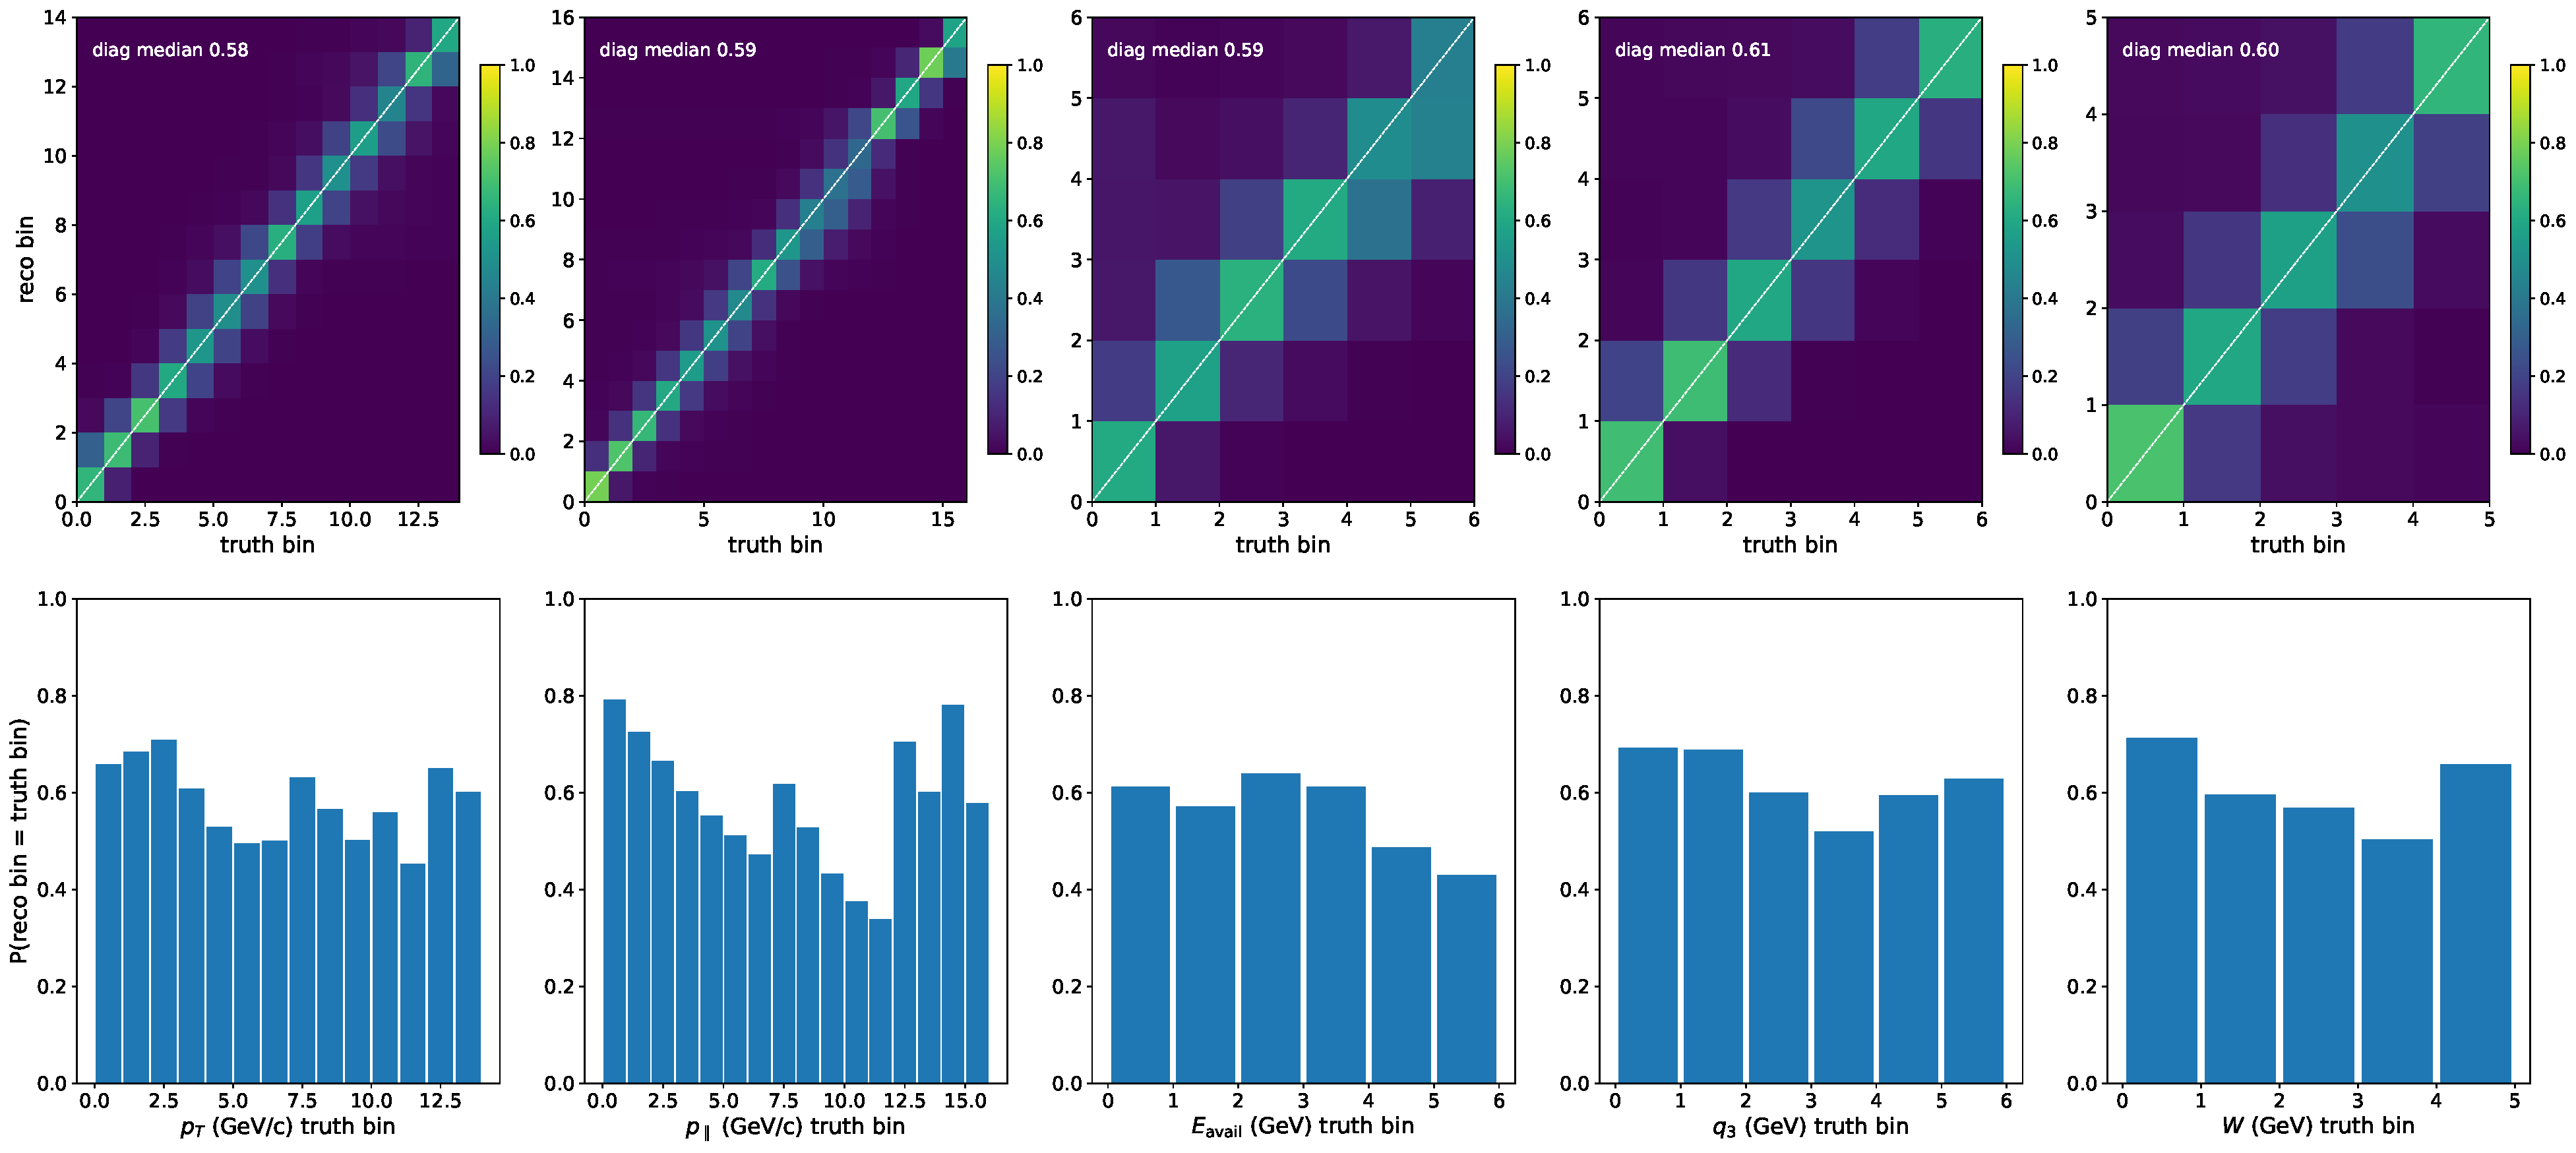
\includegraphics[width=0.8\textwidth]{migration_resolution}
  \caption{Why unfolding is needed: the detector mixes neighboring values of
  the true muon momentum together (the off-diagonal spread in these maps). A
  na\"ive bin-by-bin correction would be badly biased; unfolding undoes the
  mixing. OmniFold does it without ever building these bins.}
\end{figure}

\subsection*{What the checks tell us}

In a simulated experiment, \emph{truth} is the known answer, the \emph{prior}
is our starting prediction, and the \emph{response} describes what the detector
records for a given truth. Changing the prior changes how often simulated
events occur. Changing the response changes how those events appear in the
detector. A learner of limited capacity and a finite number of iterations can
also leave an approximation error, even with the correct response.

\begin{table}[H]
\centering\small
\begin{tabular}{@{}p{0.20\textwidth}p{0.36\textwidth}p{0.35\textwidth}@{}}
\toprule
Check & Question & What passing it does not establish \\
\midrule
Closure & Does unfolding recover a known, specified truth? & Accuracy for every other truth or detector response \\
\addlinespace
Coverage & Over repeated experiments, how often does an interval contain its target bin value? & Simultaneous coverage of all bins, or validity for a different estimator \\
\addlinespace
Bookkeeping & Are selected and missed simulated events represented consistently? & Recovery of a changed truth \\
\addlinespace
Stability & Does the answer move when iterations, seeds or rounding change? & That a stable answer is accurate \\
\bottomrule
\end{tabular}
\caption{Different checks answer different questions. Bias is a systematic
offset of the average answer from truth; a single simulated experiment can
also fluctuate. Coverage tests the estimate and its interval together.}
\end{table}

% plain-language pass, review fix RD1 (DECISION-20261018-joseph-plain-language-pass)
% plain-language pass 2 (DECISION-20261018-joseph-plain-language-pass2)
% Theme B: the PET sentences moved to "Alternative representations and signal definitions" (primer P-new-3), the
% truth-cut sentence to the signal-definition paragraph there (P-new-3), and the pointer to the selection-versus-inputs
% table (P9) to the note, which carries the table (selection_features.tex, tab:selection-features, input by
% sec_experiment.tex) and the signal-only design-study samples (its "PET design studies" row).
One more distinction matters later: which events are kept (the selection) and
what the learner is shown (its inputs) are separate choices. Every analysis of
real data here requires a reconstructed muon matched to MINOS, a second detector
downstream of MINERvA that measures the muon's momentum. The classifiers that
read summary quantities of each event use that momentum. They are
gradient-boosted decision trees, a standard machine-learning method, and from
here on we call them the \emph{tree learner}.

\section{What we found}

% plain-language pass 2 (DECISION-20261018-joseph-plain-language-pass2)
Our results have different levels of validation, so we first list each finding
with how far it has been tested. The rest of this section gives the details: the
findings, then the limits that matter most, then a separate test of five
simulations, and finally two exploratory studies.
\begin{itemize}
% plain-language pass, review fix R7, RD2 (DECISION-20261018-joseph-plain-language-pass)
% plain-language pass 2 (DECISION-20261018-joseph-plain-language-pass2)
\item \textbf{A published result, reproduced.} The two-variable central value
  (the best estimate itself, apart from its error bars) reproduces MINERvA's
  published measurement: the overall rate agrees to about one percent, although
  a shape difference remains when judged with the published correlations between
  cells. Its size depends on which of two implementations of the tree learner
  is used, and we chose which one to quote after both comparisons were known.
  Some effects are not included in its error budget, and we make no coverage
  claim for it.
  % plain-language pass, verification fix V4 (DECISION-20261018-joseph-plain-language-pass)
  The quoted statistical error bars have had no coverage test, that is, no check, on simulated repeats of the
  experiment, that they contain the truth as often as stated.
% J3/J4 provisional (DECISION-20261018, packet C4: kept): the quoted statistical block is S1 of Q = S5 total + C_PL
% (2026-10-17), untested (KNOWN_ISSUES 85, re-scoped to S1 under J5).
% plain-language pass (DECISION-20261018-joseph-plain-language-pass)
% plain-language pass, review fix R2, R4, RD3 (DECISION-20261018-joseph-plain-language-pass)
% plain-language pass 2 (DECISION-20261018-joseph-plain-language-pass2)
% Theme A (primer F-new-1): "about 10%" is the median (E_avail, W) residual, 9.7 %, under the GiBUU-to-GENIE
% E_avail-shape departure. 9.7 % median: sec_5d.tex:73; OUTCOME-20260925-s5n-stage1-development-fail.md:76.
\item \textbf{More quantities at once.} The higher-dimensional central values
  pass particular recovery checks, but they are shown as central values only.
  Other end-to-end tests show biases that are not included in their quoted
  uncertainty: when the simulated truth is changed by a test pattern of the size
  of a difference between generators, typical cells come back about
  \SI{10}{\percent} off, and the background removal leaves a bias in some cells.
  That uncertainty has not met the requirements we set in advance, and it is used
  only under a documented exception to them, so their error bars have not been
  shown to be right. The one direct test of whether such error bars contain the
  truth as often as stated, made on a variant of the method, failed. No
  significance is assigned to their differences from the simulations, because
  the uncertainty depends measurably on the learner's random seed.
% plain-language pass 2 (DECISION-20261018-joseph-plain-language-pass2)
\item \textbf{Known and new features in the data.} In these central values, all
  four tested simulations fall short of the data at low available energy,
  resembling an established low-recoil discrepancy. Adding a two-nucleon
  process fills part of the gap, without uniquely establishing the cause. The
  excess over MINERvA's tuned simulation is concentrated in one corner, at high
  available energy and high hadronic mass. Neither feature is assigned a
  statistical significance.
% plain-language pass, review fix R6 (DECISION-20261018-joseph-plain-language-pass)
% plain-language pass 2 (DECISION-20261018-joseph-plain-language-pass2)
\item \textbf{A joint test of five simulations.} This is a separate inference
  from the measurements, a test of the simulations rather than a new measurement
  with new error bars. Under stated modelling assumptions and six stated
  conditions, each of five widely used simulations, in the hybrid form defined
  below, is rejected at a combined error level of five percent, both overall and
  in shape alone. The two conditions that matter most are that the test has no
  uncertainty for the calorimeter's response to the hadronic recoil energy, and
  that the possible error from structure finer than the test's grid is not
  bounded. The test does not show that the five quantities together discriminate
  better than matched coarse projections of them.
% plain-language pass 2 (DECISION-20261018-joseph-plain-language-pass2)
\item \textbf{A neural network on raw detector data.} PET, a neural network that
  reads the individual energy deposits in the detector, remains method
  development. Simulation studies improved how well it recovers deliberately
  changed distributions, but no design met every requirement fixed in advance,
  and PET contributes no cross section or error bar.
% plain-language pass, review fix R5 (DECISION-20261018-joseph-plain-language-pass)
\item \textbf{A wider signal definition.} Relaxing the published cuts on the
  true muon's motion, with the same event selection, enlarges the population
  being estimated without adding measured events. The central value is
  preliminary: only part of the rate is newly supported by the detector, and a
  larger part is a separately labeled, simulation-dependent extrapolation.
\end{itemize}
% plain-language pass, review fix RD4 (DECISION-20261018-joseph-plain-language-pass)
Each result is only as validated as its own checks.

\subsection*{First, a trust check: reproduce a known result}

Before trusting a new method, one must show it reproduces an established
measurement. MINERvA already published this muon cross section using the
traditional method. Our machine-learning result agrees with it closely: the
overall interaction rate matches to about one percent (ratio $\ratioTot$), and
\SI{\binsTen}{\percent} of the individual measurement cells agree within ten
percent. Judged with the published correlations between cells, a shape difference
% plain-language pass, director ruling on base defect F11 (DECISION-20261018-joseph-plain-language-pass; PLAIN-LANGUAGE.md C7)
remains. Just as important, our \emph{uncertainties} --- worked out
independently of the published analysis --- come out close in size to the published ones
(\SI{\uqMedian}{\percent} versus \SI{\uqPaper}{\percent} typical). Ours are a little smaller in the typical cell,
% \uqMedian = 6.45, rebuild/outputs/outA/budget_Q.json.gz Q.median_pct (Q = S5 total + C_PL); still below \uqPaper.
% J3/J4 provisional (DECISION-20261018, packet W3: D5 is in the paper and note; the primer names no run-period block).
% plain-language pass (DECISION-20261018-joseph-plain-language-pass)
partly because our uncertainty on the beam's neutrino flux comes out below the
published one, for a reason not yet established; both use MINERvA's constraint
from neutrino--electron scattering and inverse muon decay. For the uncertainty
on the overall interaction rate the comparison goes the other way:
\SI{\uqIntegral}{\percent} for ours against \SI{\uqPaperIntegral}{\percent}
published.
% J3/J4 provisional (DECISION-20261018, packet C2: the per-bin median and the integral; W7: the flux sentence kept;
% W5: the "earlier version ... 6.87 percent" clause dropped, the chain is in the note's App. history).
% \uqIntegral = budget_Q.json.gz Q.integral_sigma_pct (4.755); \uqPaperIntegral = 4.61 (values.tex).
% plain-language pass (DECISION-20261018-joseph-plain-language-pass)
The new method reproduces the old answer, and its error bars are close in size
to the published ones.

One qualification: two software implementations of the tree learner give
answers that differ by about one percent in a typical cell, and the size of the
remaining shape difference depends on which one is used. We quote the faster
one, because every ingredient of the error bars was computed with it; we had
originally quoted the slower one. We made this choice after both comparisons with the
% J3/J4 provisional (DECISION-20261018, packet W3: D5 not in the primer): the run-period block is built from seed-42
% per-period unfolds of the same pipeline (period-unfold REPORT §1).
% plain-language pass (DECISION-20261018-joseph-plain-language-pass)
published result were known.

% plain-language pass 2 (DECISION-20261018-joseph-plain-language-pass2)
% Theme B (primer P1): the list of repaired defects moved to the note, sec_systematics.tex sec:uq-2d-construction
% (the May-sweep truth-input mismatch, the Rvn1pi/Rvp1pi double count, the background-template statistics, the
% selection-complete lateral re-unfolds); the paper keeps its version in sec:uq2d.
The error budget also has known limits. An assessment of the saved analysis
outputs found errors in how an earlier version of the two-variable error budget
was put together~\cite{TwoDFollowup2026}. The quoted budget was rebuilt without
them; the analysis note lists the repairs. Some effects are not
included in any part of the budget: an approximation in how events that fail
reconstruction are weighted, the difference between the two implementations of
the tree learner, and the dependence on the unfolding model.

To test whether error bars have the right size, one reruns the analysis on many
simulated experiments and counts how often the bars contain the known answer
(their \emph{coverage}). Making those experiments by splitting the simulation we
already have can test the precision for that particular sample, but it cannot
establish coverage across independently generated samples. Validated error bars
would need new inputs: an independent simulation of full size, a validated way to
generate variations of the uncertain model parameters (nuisance variations), and
samples from independent generators that have not already been inspected. We
make no coverage claim.
% J3/J4 provisional (DECISION-20261018, packet C3, applied here after review M1, director's ruling 2026-10-18): the
% paragraph said the budget "needs construction repairs" and "has not been recalculated", false of Q. Q uses the July
% sweep (no truth-input mismatch; sec_systematics sec:uq-2d-construction; stageC/production/DESIGN.md §S5 universe row),
% drops Rvp1pi (KNOWN_ISSUES 92), draws a background bootstrap stream (S1, DESIGN §3.4), takes its laterals from
% selection-complete re-unfolds (S3), and was recalculated (stageF/rebuild/REPORT.md §3). The flux-universe index
% identity is established (KNOWN_ISSUES 91; Stage B REPORT §2.1), so "matching flux variations need further
% verification" is removed. Exclusions: DECISION-20261017 §2 (G2, the learner dependence, C09); the new inputs and "no
% coverage claim": DECISION-20261014 §2. The paper's version is paper_body.tex sec:uq2d (C3).
% plain-language pass (DECISION-20261018-joseph-plain-language-pass)

% plain-language pass, review fix R13 (DECISION-20261018-joseph-plain-language-pass)
We did run such a test on the statistical part of those error bars, using
simulated repeats drawn from our own simulation against a fixed, known truth.
The answer is uneven. In
many cells the bars are about right or even too wide. In a block of cells with
large forward momentum, and in those with the largest sideways momentum, they
are too narrow. Pooled over all cells, two-standard-deviation bars contain the
truth \SI{\covTwoDCTwoPct}{\percent} of the time instead of \SI{95}{\percent}.
% plain-language pass, director ruling on base defect note F2 (DECISION-20261018-joseph-plain-language-pass; PLAIN-LANGUAGE.md C7)
That test was of the statistical error bars in use when it ran. The main cause of
the shortfall was found and removed, and the statistical bars now quoted were
built again, at the same learner settings as the central value. They have not
been tested.
% J3/J4 provisional (DECISION-20261018, packet C4: kept; W3: D2, D10 KI-88 in the paper and note): S1, 300 replicas at
% seed 42 (stageC/production/DESIGN.md S3.4); untested (KNOWN_ISSUES 85).
% plain-language pass (DECISION-20261018-joseph-plain-language-pass)
The published numbers are unchanged by this check.

% plain-language pass 2 (DECISION-20261018-joseph-plain-language-pass2): placement [tbp], so the near-full-page figure
% no longer leaves the preceding page half empty.
\begin{figure}[tbp]
  \centering
  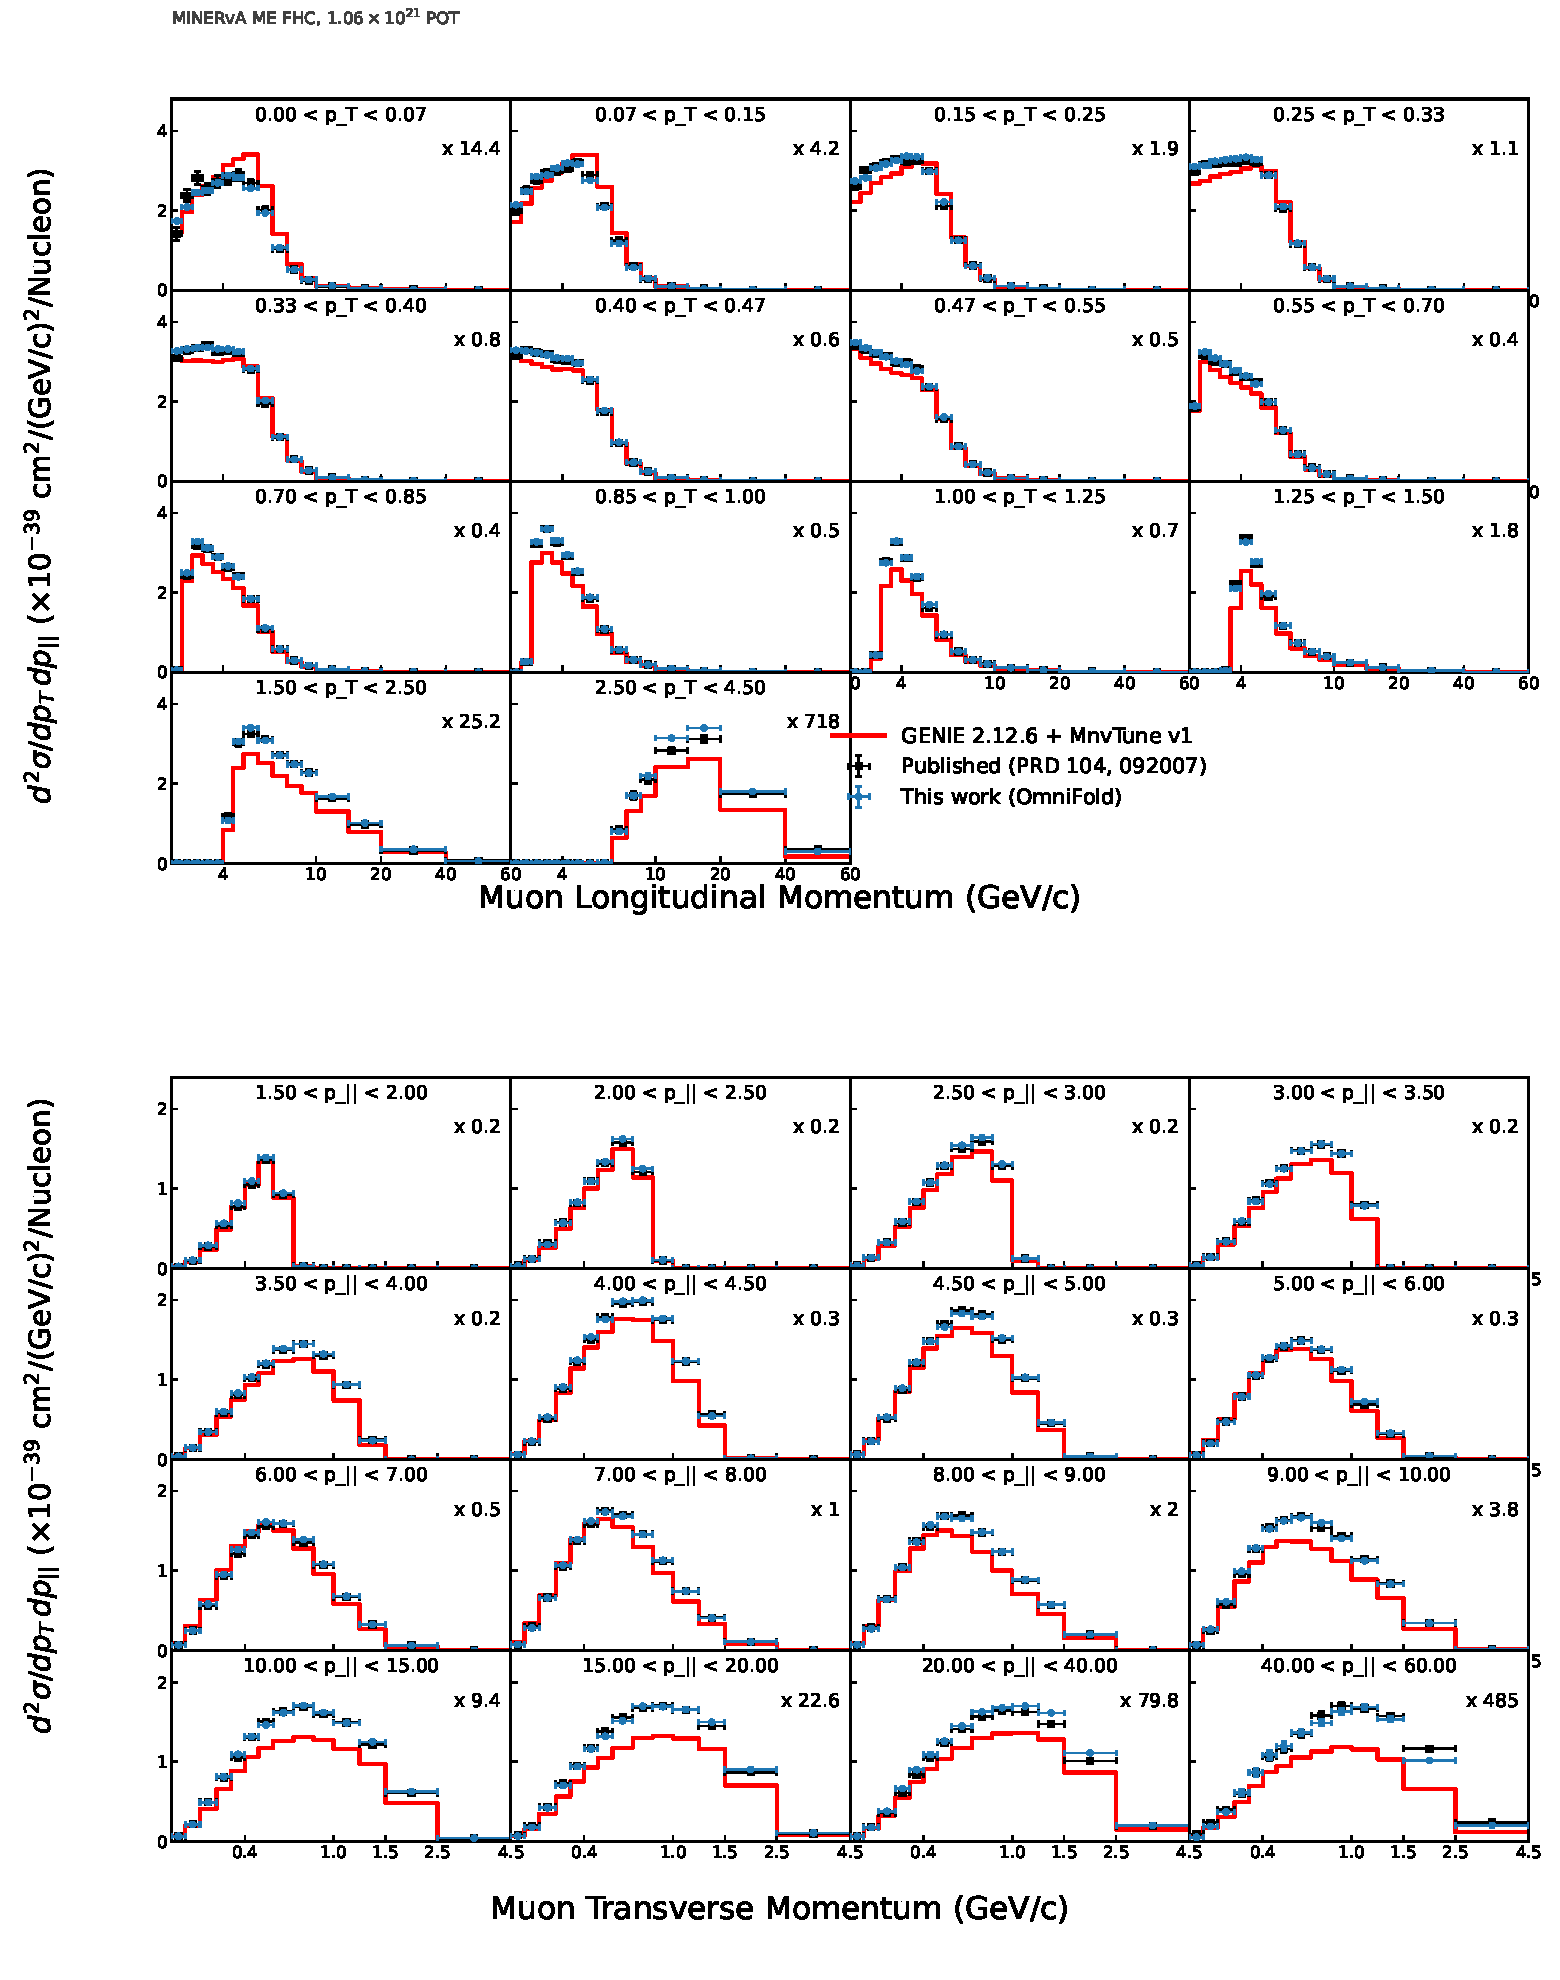
\includegraphics[width=0.62\textwidth]{MEFHC_5iter_fig13}
% plain-language pass 2 (DECISION-20261018-joseph-plain-language-pass2)
% Theme A (primer F-new-8): legend "GENIE 2.12.6 + MnvTune v1", color red, in 2d-unfolding/plot_2d_threeway_fig13.py:200
% (called by make_figures.sh:35); paper_body.tex:110-111; note sec_experiment.tex:24.
  \caption{The unfolded muon cross section as a function of the two momentum
  components. This reproduces a published MINERvA measurement, but was produced
  by the machine-learning method described above. The red curve is MINERvA's
  tuned simulation (Tune~v1, built on GENIE~2.12.6), the starting point of the
  unfolding; the untuned GENIE~2.12.10 of Fig.~\ref{fig:primergen} is a
  different simulation.}
\end{figure}

\subsection*{Then, measure more at once --- and rediscover known physics}

% plain-language pass, director ruling on base defect F3 (DECISION-20261018-joseph-plain-language-pass; PLAIN-LANGUAGE.md C7)
% plain-language pass, review fix R3 (DECISION-20261018-joseph-plain-language-pass)
With the central value reproduced, and its error bars found close in size to
the published ones, we used OmniFold's defining ability and unfolded
several quantities \emph{simultaneously} and \emph{without binning} --- a first
at MINERvA, where earlier multi-quantity results used binned methods: the muon
momentum together with the available energy ($\Eavail$, roughly how much energy
the struck nucleus released), the momentum transfer ($q_{3}$), and the hadronic
mass ($W$).
% plain-language pass, review fix N1, director instruction: normalization agreement only (DECISION-20261018-joseph-plain-language-pass)
Each richer measurement, when collapsed back down, agrees with the simpler one
in overall normalization --- a built-in consistency check.

These are five recorded coordinates, not five demonstrated independent pieces
of information. The reconstructed momentum transfer and hadronic mass reuse
the muon's motion and the same recoil-energy estimate. Available energy is
a different quantity: in particular it omits energy carried by neutrons at
truth level. A new coordinate can help the learner describe correlations
without revealing a new independently measurable direction.

The first physics payoff appears in the available energy. When we compare the
data to four state-of-the-art simulation predictions, all four fall short of
the data in the low-energy region, just above the very lowest energies
(Fig.~\ref{fig:primergen}, left). This is not a
surprise --- it resembles an established low-recoil discrepancy that simulations
have historically struggled to model. Adding a process in which the neutrino
interacts with a pair of nucleons (``2p2h'') fills part of the gap. The two tested
pion-rescattering variations have a much smaller effect, but that does not rule
out other changes to how particles move through the nucleus. Related MINERvA
measurements with a different event selection show why proton and pion
rescattering also matter~\cite{MINERvA:2026qeleme}. These comparisons support the
two-nucleon contribution without uniquely establishing the cause. And
where MINERvA has a dedicated published measurement of this region, our central
values lie \SI{9.2}{\percent} and \SI{6.3}{\percent} above it on the finest grid
whose cell edges both measurements share.
% plain-language pass, director ruling on base defect F6 (DECISION-20261018-joseph-plain-language-pass; PLAIN-LANGUAGE.md C7)
That measurement defines true available energy more broadly, so this comparison
is not quantitative.

\begin{figure}[H]
  \centering
  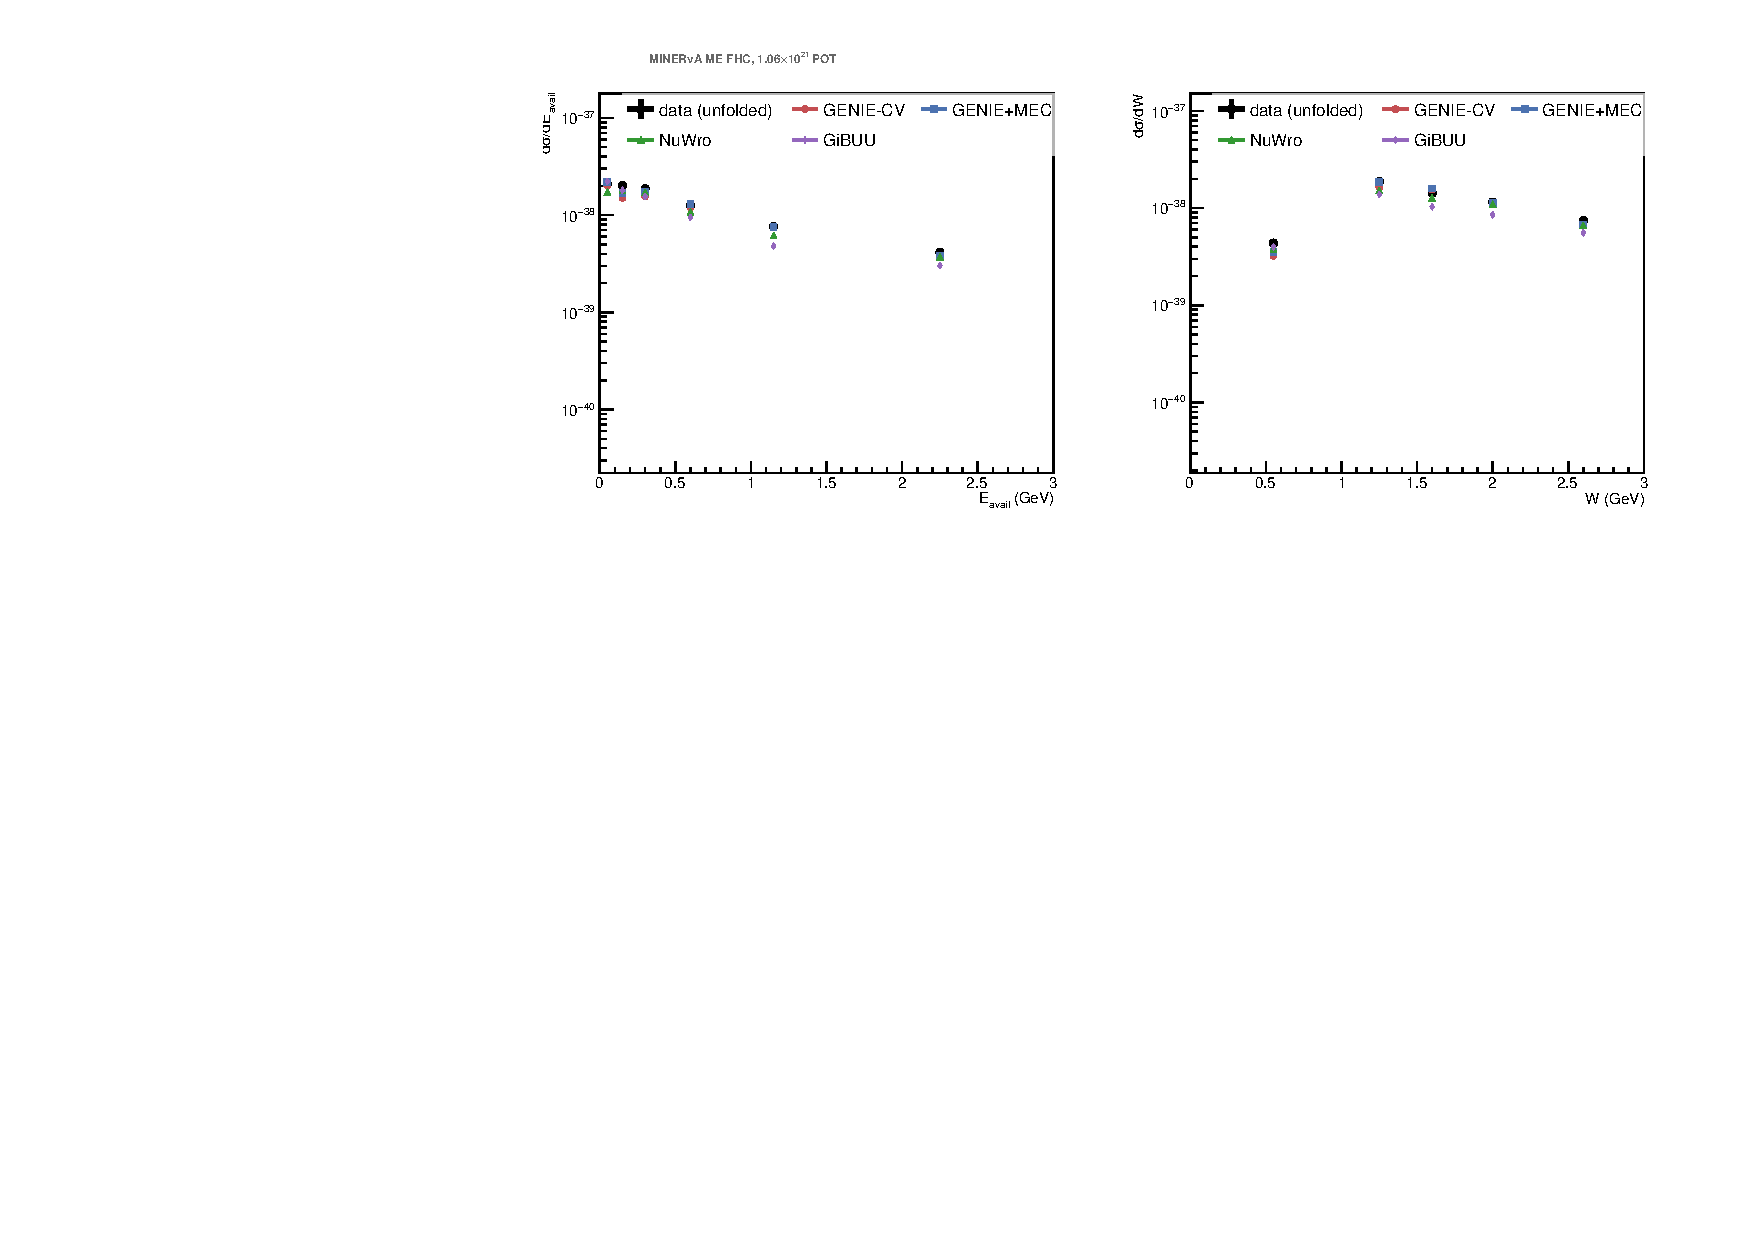
\includegraphics[width=0.99\textwidth]{eavailW_band}
% plain-language pass 2 (DECISION-20261018-joseph-plain-language-pass2)
% Theme B (primer P8): the clause "the GENIE and NuWro predictions were rebuilt with a correctly sampled beam
% spectrum" moved to the note, sec_3d.tex (flux-repaired predictions, l.239-245) and sec_eavailw.tex (l.97-98, l.139).
  \caption{The unfolded central values (black points) compared to four tested
  simulation predictions --- GENIE's own untuned central configuration (version 2.12.10), the same GENIE
  with the two-nucleon process added, NuWro (21.09) and GiBUU (2019). \emph{Left:} available
  energy; all four fall below the data at low available energy (between about
  $0.1$ and $0.4$~GeV), the known
  ``low-recoil'' shortfall, here rediscovered by a different unfolding method.
  \emph{Right:} hadronic mass; all four sit below the data at high hadronic
  mass, the first three by about as much as they fall short overall. \textbf{Central values only.} No uncertainty band is drawn and no
% plain-language pass, review fix R10 (DECISION-20261018-joseph-plain-language-pass)
  significance is assigned, for the reason given under ``Limits on the
  multi-quantity results'' below.
  The first two predictions are two configurations of the same generator and
  are not independent of each other.}
  \label{fig:primergen}
\end{figure}

\subsection*{A new puzzle for the tuned simulation}

% plain-language pass 2 (DECISION-20261018-joseph-plain-language-pass2)
% Theme A (primer F-new-2): shares of the cell-integrated positive excess over Tune v1: 67 % at E_avail >= 0.8 GeV,
% 83 % of that at W >= 1.8 GeV, 22 % in the E_avail > 3 GeV, W > 3 GeV catch cell. Note sec_eavailw.tex:49-53;
% paper_body.tex:571-574 (the 22 % from the released figure arrays, fig_arrays.npz sha256 72394a2b...).
Adding the hadronic-mass axis $W$ lets us look where MINERvA's tuned simulation,
which already includes an enhanced two-nucleon process, still misses. The
leftover discrepancy sits
in a specific corner: high available energy \emph{and} high $W$ --- the
``deep-inelastic'' region where the neutrino shatters the nucleon. Of the extra
cross section, summed over cells, about two thirds lies at high available
energy, most of it at high $W$, and about a fifth sits in the single widest
corner cell. That corner
is a statement about the two quantities \emph{jointly}, so
Fig.~\ref{fig:primerjoint} shows the joint map rather than the two separate
one-dimensional views of Fig.~\ref{fig:primergen}: neither of those alone
would show it. The four other simulations also fall short of the data there,
but three of them (the two GENIE versions and NuWro) fall short by roughly as
much as they do everywhere: the data are \SIrange{14}{16}{\percent} above them
in the corner and \SIrange{7}{15}{\percent} above them overall, so for them the
corner is not a special place. GiBUU falls much further behind there (the
data are \SI{61}{\percent} above it in the corner, \SI{39}{\percent} overall), but mostly
because its simulated sample leaves out neutrinos above \SI{20}{GeV}, which in the other
simulations make up about \SI{15}{\percent} of the corner and \SI{7}{\percent} of everything.
With them supplied, GiBUU too falls short in the corner by about as much as overall.
% plain-language pass 2 (DECISION-20261018-joseph-plain-language-pass2)
% Theme A (primer F7): \cvMoveOverSigmaMax = 6.02 (values.tex:458; CENTRAL-VALUE-VS-SIGMA-20260920.json
% movement_over_uncertainty.max 0.0602), printed rounded to the nearest percent by siunitx (prints 6).
Its statistical significance is not assigned. The learner's random seed,
% plain-language pass, review fix R10 (DECISION-20261018-joseph-plain-language-pass)
described under ``Limits on the multi-quantity results'' below, moves these central values as well, by at most about
\SI[round-mode=places,round-precision=0]{\cvMoveOverSigmaMax}{\percent} of their own uncertainty; how far the
corner's share of the excess could shift with it was not separately measured.
% plain-language pass 2, director ruling on F-p2-1 and F-p2-2 (DECISION-20261018-joseph-plain-language-pass2; PLAIN-LANGUAGE.md C7): the
% corner carries the paper's caveat (paper_body.tex at 34650231, l.577-580: no mismodelled-response closure for this map; largest
% regularization bias there), and "points theorists toward what their models are missing" is cut as stronger than the body supports.
No test with a deliberately wrong detector response has been run for this map,
and this corner is also where the unfolding's bias toward its starting
simulation is largest. The localized difference was only visible because we
measured available energy and $W$ jointly.

\begin{figure}[H]
  \centering
  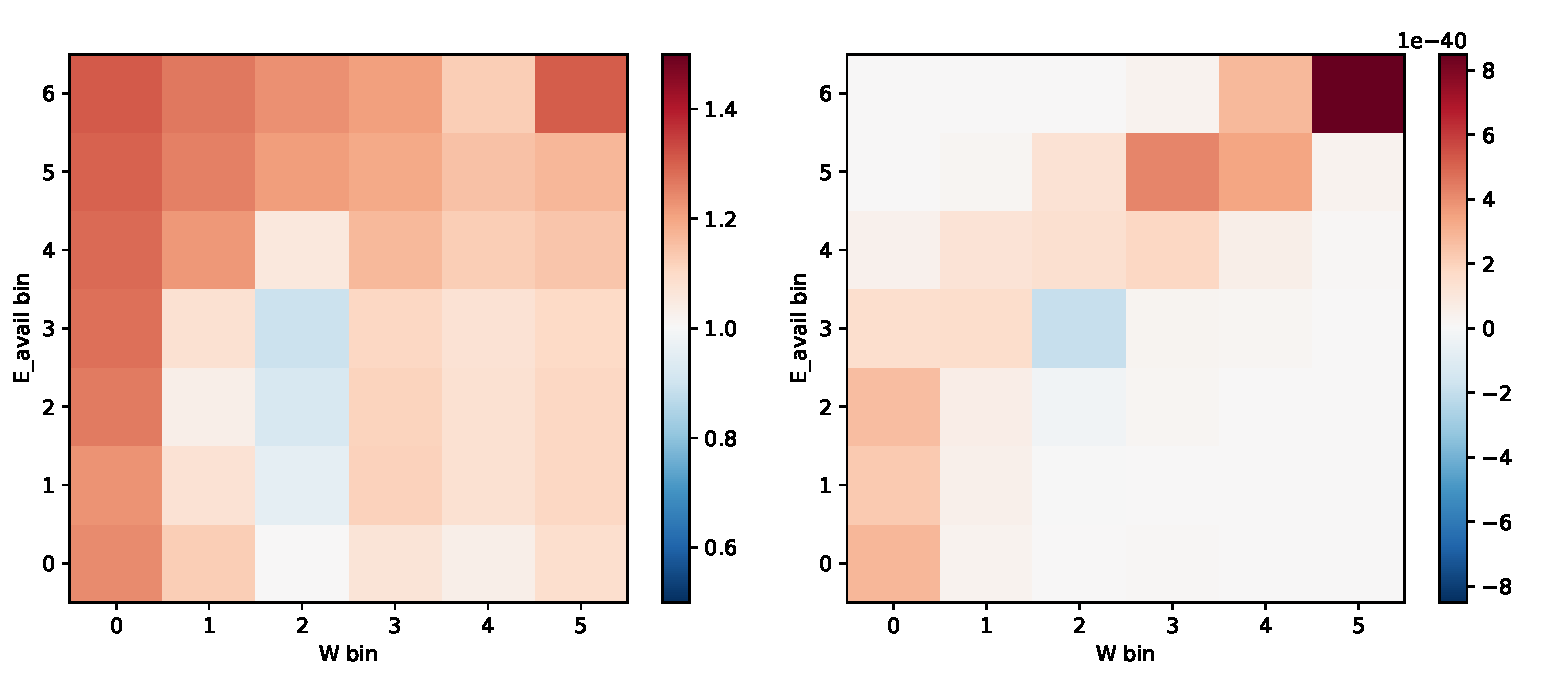
\includegraphics[width=0.95\textwidth]{paper_joint_localization}
% plain-language pass 2 (DECISION-20261018-joseph-plain-language-pass2)
  \caption{The unfolded data compared to the MINERvA-tuned GENIE simulation (MINERvA Tune~v1, the simulation the unfolding starts from, not the untuned ``central configuration'' of Fig.~\ref{fig:primergen}) across
  the available-energy / hadronic-mass plane \emph{jointly}. Both panels are
  measured on the same seven-by-six grid of cells, with available-energy
  boundaries $0$, $0.1$, $0.2$, $0.4$, $0.8$, $1.5$, $3$ and $100$~GeV and
  hadronic-mass boundaries $0$, $1.1$, $1.4$, $1.8$, $2.2$, $3$ and
  $100$~GeV; the axes are labelled by cell number, counting from zero, and the
  last cell on each axis is a wide catch-all that collects everything above
  $3$~GeV. \emph{Left:} the ratio of data to simulation, so $1$ means
  agreement. \emph{Right:} the difference, data minus simulation, as a
  cross section \emph{integrated over each cell}
  (\si{cm^2/nucleon}) --- because that includes the cell's area, the wide
  catch-all cells look large here even where the ratio on the left is
  moderate, and the two panels should be read together. The excess concentrates
  in the top-right corner: high available energy \emph{and} high hadronic mass.
  Central values only; no uncertainty is drawn and no significance is assigned.
  The learner's random seed moves these central values by at most about
  \SI[round-mode=places,round-precision=0]{\cvMoveOverSigmaMax}{\percent} of their own uncertainty.}
  \label{fig:primerjoint}
\end{figure}

% plain-language pass, review fix R10 (DECISION-20261018-joseph-plain-language-pass)
\subsection*{Limits on the multi-quantity results}

% plain-language pass, review fix RD3 (DECISION-20261018-joseph-plain-language-pass)
% plain-language pass 2 (DECISION-20261018-joseph-plain-language-pass2)
The multi-quantity central values above pass the validation tests stated with
them. Three limits matter most, in this order. First, the unfolding follows a
changed simulated truth only partly, which leaves biases that are not in the
quoted uncertainty. Second, that uncertainty has not met the requirements we
set in advance, and it depends measurably on the learner's random seed. Third,
a test of numerical stability, fixed in advance, failed. The multi-quantity
plots therefore show central values only, and we do not assign statistical
significance to their differences from the simulations.

% plain-language pass 2 (DECISION-20261018-joseph-plain-language-pass2)
% Theme B (primer P7): the wrong beam-spectrum sampling behind the test pattern moved to the note, sec_5d.tex
% sec:val-fiveaxis "Generator-sized truth changes" (l.67-71: "mis-sampled flux ... not a measured GiBUU--GENIE
% difference"); the primer keeps that it is not a measured difference between generators.
\emph{Biases in following a changed truth.} When the simulated ``true''
distribution of available energy is changed by a test pattern of the size of a
difference between two standard generators (a test of chosen size, not a
measured difference between them), the unfolding follows it only partly.
Typical cells come back about \SI{10}{\percent} off, and the highest-$W$ cells
much more. The tested changes to the number of iterations and to the learner's
capacity do not remove the bias; their effects depend on the injected truth and
the quantity reported. For test patterns from other generators the effect is
\SIrange{16}{31}{\percent} in the worst cell and smaller than the quoted
uncertainty in about half of the $(\Eavail,W)$ cells. This dependence on the
truth is not included in the quoted uncertainty. A second end-to-end test
includes background in the simulated pseudo-data and processes them exactly as
the data are: the way we remove background biases the highest-$W$ cells by
about \SI{4}{\percent}. A finer, unbinned removal cuts that to below
\SI{0.3}{\percent}, but leaves about \SI{1}{\percent} in a few combined cells.
A follow-up study found the source of this remaining bias: an auxiliary
classifier used in the background removal was too simple, and a larger one
removes the bias. Neither effect is in the quoted uncertainty yet.
% plain-language pass, review fix RD7 (DECISION-20261018-joseph-plain-language-pass)
% plain-language pass 2 (DECISION-20261018-joseph-plain-language-pass2)
% Theme B (primer P6): the remedies are compressed to one sentence; the note carries them in sec_5d.tex
% "Variability and interval behavior at five iterations" (no tradeoff; coarser cells estimate different integrals)
% and the prior-shift paragraph ("no ... guaranteed bias bounds").
Three possible remedies each have a limit: longer runs sometimes improve
recovery, but how much they vary from one repeat to the next was not measured
at the same settings, so no tradeoff between bias and variability is
established; combining cells changes what is measured; and changing the
starting model gives no guaranteed error bound.
% plain-language pass, review fix R1 (DECISION-20261018-joseph-plain-language-pass)
None of these studies changed the five-quantity central value or its quoted
uncertainty.

% plain-language pass 2 (DECISION-20261018-joseph-plain-language-pass2)
% Theme A (primer F7): \sprojMeasured = 6.145 (values.tex:407; GRADE-20260920-cause3-two-member.json s_proj
% 0.06145), printed rounded to the nearest percent by siunitx (prints 6); \sprojBound = 5 (values.tex:408).
\emph{An uncertainty that has not been validated.} We have built an
uncertainty for the five-quantity result, and the two-quantity $(\Eavail,W)$
version of that uncertainty. It is the uncertainty we quote for the
five-quantity result, but it has not met the requirements we set in advance, so
it is used only under a documented exception to them. The reason we assign no
significance is worth stating plainly, because it is something we measured
rather than a precaution. Our method has a random component: the learner is
started from a random seed. Change that seed, leaving everything else alone, and
the \emph{uncertainty} we report on the $(\Eavail,W)$ projection shifts by
about \SI[round-mode=places,round-precision=0]{\sprojMeasured}{\percent}, more
than the \SI{\sprojBound}{\percent} we had decided in advance we would
% plain-language pass, review fix RD3 (DECISION-20261018-joseph-plain-language-pass)
tolerate. That was measured on two test versions of the uncertainty built for
exactly this comparison, not on the one we quote. The shift is the same size
whether we use a quarter, a half, or all of our simulated variations, while
genuine statistical noise, measured between the quarter and the half, falls by a
factor of nearly three over the same step, so it behaves like a real property of
the learner rather than like noise. We compared only one pair of random seeds,
however, and nested subsets of one set of variations cannot rule out what a
much larger set would give. Five of the forty-five uncertainty components are
built with a fixed seed that this change cannot reach, and we have not measured
which way those five would move the shift. The same seed change moves the
\emph{central values} too, though only by at most about
\SI[round-mode=places,round-precision=0]{\cvMoveOverSigmaMax}{\percent} of their
own uncertainty. Reporting a significance on top of that would claim a
precision the input does not have. Finally, the one direct test of whether
five-quantity statistical error bars contain the truth as often as stated was
made on a variant of the method, and it failed, so we claim no such coverage.

% plain-language pass, review fix R12, RD6 (DECISION-20261018-joseph-plain-language-pass)
% plain-language pass, director ruling on base defect F4 (DECISION-20261018-joseph-plain-language-pass; PLAIN-LANGUAGE.md C7)
% plain-language pass 2 (DECISION-20261018-joseph-plain-language-pass2)
\emph{Numerical stability.} The follow-up study also found that the result on
the real data shifts by up to a few times its statistical uncertainty when the
inputs are rounded differently, which fails a stability test fixed in advance.
A later study found that the bootstrap of the version of the method with the
larger classifier (its own resampling estimate of its statistical error)
already carries this rounding variability.
That finding is limited to that version's own bootstrap: it does not carry over
to the uncertainty quoted for the five-quantity central value,
and the stability test still counts as failed.

% plain-language pass, review fix RD5 (DECISION-20261018-joseph-plain-language-pass)
% plain-language pass 2 (DECISION-20261018-joseph-plain-language-pass2)
A narrower point concerns what the detector uncertainties cover. Five of them
describe effects that move a muon's measured momentum or angle, and for those we
rebuilt the simulation end to end so that events crossing into or out of the
selection are counted properly. Four others --- the efficiency of MINOS for the
muon, and three describing how hadrons interact in the detector --- are applied
instead by reweighting the simulated events, so there is nothing to rebuild.
By itself, that says nothing about whether the hadronic-response variations we
include are the complete set this measurement needs.

None of these five-quantity findings affects the two-dimensional trust check,
which retains its independently constructed uncertainty, with the qualification
about learner dependence explained there.

\subsection*{A joint test of five simulations}

We also asked a sharper question: under stated modelling assumptions, is each
of five widely used simulations (MINERvA Tune~v1, GENIE with and without MEC,
NuWro, GiBUU) statistically compatible with the five-dimensional data, both
% plain-language pass, review fix R11, RD8 (DECISION-20261018-joseph-plain-language-pass)
% plain-language pass 2 (DECISION-20261018-joseph-plain-language-pass2)
overall (rate and shape together) and in shape alone? Here MEC (meson-exchange
currents) labels GENIE with its model of the two-nucleon process added, and
Tune~v1 is MINERvA's tuned simulation, the one the unfolding starts from.
Strictly, each hypothesis is a hybrid: it sets the true cross section, in each
cell of a finite grid of true values, to that generator's rate, with Tune~v1's
shape inside each cell. The unfolding still learns from unbinned
events; the grid specifies the hypothesis and the quantities tested.

% plain-language pass 2 (DECISION-20261018-joseph-plain-language-pass2)
% Calibration sentences: paper_body.tex sec:joint ("The null distribution of each statistic is obtained from
% pseudo-experiments that run the full analysis chain at the null truth"; "The metric influences each test's power;
% the null calibration determines its size"; the estimator's pull toward its prior is reproduced) and
% sec:uncertainty-status (the five-dimensional covariance "is separate from the joint-test calibration").
Rather than rely on a textbook formula for how the test statistic is distributed, we
simulated about 1,340 to 1,750 pseudo-experiments (simulated repeats of the
experiment) under each simulation's hypothesis, unfolded each one through the
full analysis, and counted how often one looked as discrepant as the data.
Because each pseudo-experiment repeats the whole analysis, including the
unfolding's pull toward its starting simulation and the modelled uncertainties,
these repeats set how often the test would wrongly reject a true hypothesis.
The test therefore does not rely on the five-quantity error bars described
above, which were built separately; the matrix used to weigh the differences
affects only how sensitive the test is. In each test at most one
pseudo-experiment looked as discrepant as the data.
So all ten hypotheses (five simulations, each tested overall and in shape) are
rejected at a combined 5\% error level for the ten tests, as the test was
designed. Some pseudo-experiments were lost to computing time limits.
Rerunning exactly those seeds recovered them, in a check reported separately
from the result: none looked as discrepant as the data, though in one
robustness variant one came close.

% plain-language pass 2 (DECISION-20261018-joseph-plain-language-pass2)
% Theme B (primer P4, P5): the six-item list moved to the note's sec_joint.tex sec:joint5d-conditions (the six
% conditions, grouped by kind) and the kappa scan (the multiplier's meaning, the first loss of a determinate
% rejection near 5.26, or 5.17 with the recovered draws) to sec:joint5d-kappa; the paper keeps them in
% sec:conditions and its Results. Every condition stays named here.
This is a test of the simulations under six conditions, detailed in the analysis
note (``Joint five-dimensional generator tests''). Two matter most for what the
rejections mean physically. The detector-uncertainty model has no uncertainty
band for the calorimeter's response to the hadronic recoil energy, so the
rejections are conditional on the simulation's hadronic response. And the test
does not resolve structure finer than its grid: convergence as the grid is
refined has not been shown, and the possible error from that finer structure is
not bounded.
% plain-language pass, review fix RD9 (DECISION-20261018-joseph-plain-language-pass)
A sensitivity scan probes this error in one direction only and
gives no bound on it. The other four conditions are the interaction-model
variations as stated, including the clipping of some negative event weights; a
calibration shift, with a stated bound, that arises because the
pseudo-experiments use half the simulation and the data unfolding uses all of
it; the range of neutrino energies each generator covers; and the finite size of
each generator's simulated sample. Sensitivity to numerical rounding is also
checked. The result is not a new measurement with new error bars.

In a comparison chosen after the result was known (post hoc), GENIE's untuned
central configuration (GENIE CV) is not rejected on the same coarse projection
onto the muon variables alone, whereas its projection onto the hadronic
variables is rejected. Hadronic information therefore takes part in this rejection, but we did not
establish that the joint five-variable test adds power beyond all the matched
lower-dimensional projections. A simulation that is not rejected is not thereby
accepted as true.
% Source: docs/orchestration/RECORD-20261005-s5p-joint-5d-inference-result.md; DECISION-20261005 section 5.
% Wording review: docs/orchestration/REVIEW-20261006-s5p-stage7-note-wording.md.

\subsection*{Alternative representations and signal definitions}

Two studies test the method's limits rather than adding to the measurement.

% plain-language pass 2 (DECISION-20261018-joseph-plain-language-pass2)
% Theme B (primer P-new-3): the PET description moved here from Sec. 2.
PET is a different learner from the tree learner: a neural network (a
``point-cloud transformer'') that reads the individual energy deposits in the
detector rather than summary quantities. The original version of PET reads only
the hadronic recoil (the energy deposited by particles other than the muon), so
it does not use the muon, even though the muon is needed to select the event.
It shows that the machinery runs end to end on low-level detector data,
pairing reconstructed recoil clusters with the hadrons in the simulated true
final state. Because the muon was withheld from both of its classifiers, this
is a recoil-only diagnostic and a method-development cross-check, not a
measurement of the whole event. A later, full-event version of PET also reads
the muon; it too is method development only.

% plain-language pass, review fix RD10 (DECISION-20261018-joseph-plain-language-pass)
% plain-language pass, review fix RD10 (DECISION-20261018-joseph-plain-language-pass)
% plain-language pass, review fix R8 (DECISION-20261018-joseph-plain-language-pass)
% plain-language pass, review fix RD11 (DECISION-20261018-joseph-plain-language-pass)
% plain-language pass, review fix RD12 (DECISION-20261018-joseph-plain-language-pass)
% plain-language pass, review fix RD10 (DECISION-20261018-joseph-plain-language-pass)
% plain-language pass, review fix RD11 (DECISION-20261018-joseph-plain-language-pass)
% plain-language pass, review fix RD10 (DECISION-20261018-joseph-plain-language-pass)
% plain-language pass 2 (DECISION-20261018-joseph-plain-language-pass2)
% Theme B (primer P2): the PET design-study chronology and narrative moved to the PET note (pet_note.tex, which
% inputs sec_pet.tex and sec_pet_campaigns.tex): sec:pet-campaigns (the ten-iteration improvement study; recovery
% 0.316/0.306 for the original PET, 0.895 and 0.863 for the two finalists; the robustness failure, statistically
% unresolved; tab:pet-final-coverage, 0.896 aggregate and 0.257/0.789 at low acceptance; "What the saved intervals
% diagnose", the six-fit mean and the square-root-of-six point; member-mean coverage unmeasured on generator cases and
% at data scale), sec:pet-gbdt-paired (which learner does better per test; the binned methods on the one-dimensional
% tilt; the separate GBDT configuration) and "Where generator recovery is lost" (detector-step underfitting, weak
% extrapolation to missed events, exact weights recover the change, untested truth-level inputs).
Studies on simulated samples that contain signal events only then improved how
well PET recovers deliberately changed truth
distributions~\cite{PETImprovement2026,PETFinalDesign2026}. Better recovery was
not enough: no design met every requirement fixed in advance. One of the two
best designs failed a robustness rule, fixed in advance, for its point estimate.
The other failed the test of its error intervals, which contained the truth more
often than stated over the whole distribution and much less often than stated
where the detector records only a small fraction of the true events (low
acceptance). A diagnosis of these intervals explains part of this behavior but
gives no validated repair~\cite{PETIntervalDiagnosis2026}. An exploratory
comparison ran OmniFold with each of the two learners on exactly the same
simulated events~\cite{PETGBDT2026}. Figure~\ref{fig:primerpet} shows PET's
advantage on the two energy tilts, but the tree learner does better on all three
tests that reweight to other generator models, so which learner does better
depends on the test. This is not a general ranking of the two kinds of
unfolding, and it compares neither their precision nor the two PET designs. A
separate diagnosis locates where PET falls short on the generator-model tests,
without establishing a cause that holds in
general~\cite{PETGeneratorDiagnosis2026}. These results hold only for the
study's finite simulated samples. No design or default was selected, and no PET
uncertainty is used for any result.

\begin{figure}[H]
  \centering
  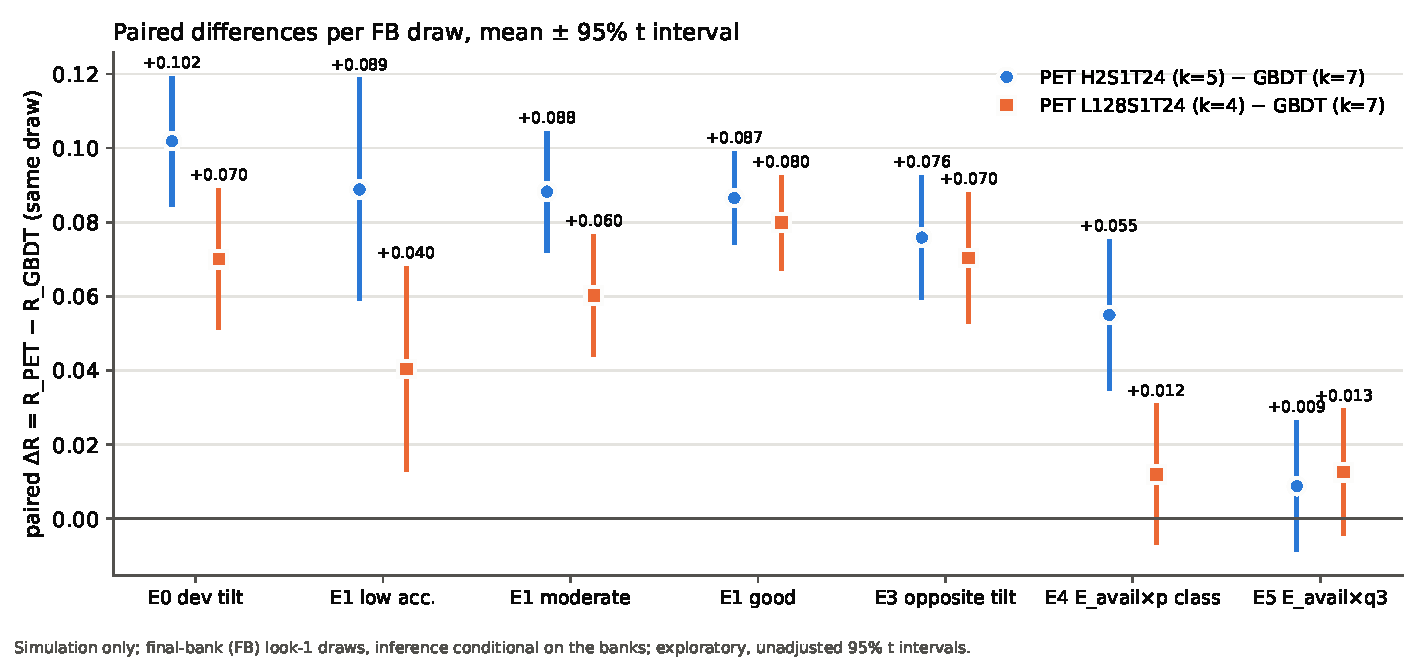
\includegraphics[width=0.90\textwidth]{pet_gbdt_paired_differences.pdf}
% plain-language pass, review fix RD10 (DECISION-20261018-joseph-plain-language-pass)
% plain-language pass 2 (DECISION-20261018-joseph-plain-language-pass2)
  \caption{Exploratory simulation comparison: gain in recovered fraction for
  each of the two best PET designs relative to the tree learner (labelled GBDT, for
  gradient-boosted decision trees, in a separate configuration from the one used
  for the five-quantity results) on the same events, at the seven iterations
  chosen in development. Positive is better recovery.
  E0 and E3 are opposite energy tilts; E1 separates acceptance regions;
  E4 tests proton content and E5 the joint energy--momentum-transfer
  distribution. Bars are unadjusted 95\% intervals for paired differences
  over 60 draws (E0, E1, E3) or 40 (E4, E5), conditional on the simulated
  samples. These are point-estimate comparisons, not validated uncertainty bands.}
  \label{fig:primerpet}
\end{figure}

% plain-language pass 2 (DECISION-20261018-joseph-plain-language-pass2)
% Theme A (primer F7): \fpsSigma = 4.502e-38 (values.tex:273; VALIDATION_LEDGER.md:1615; three-prior values
% 4.502/4.475/4.367e-38 at :1625), printed to two significant figures by siunitx (prints 4.5 x 10^-38).
Separately, the published signal definition excludes about a third of the
simulated interaction rate because of its muon kinematic cuts. This fraction
is a simulation estimate, not a measured number. We relaxed those truth-level
cuts while retaining the same tracker interaction volume and reconstructed
MINOS-based selection. Removing these cuts enlarges the population being
estimated without adding selected observations. The preliminary central value
of the extended cross section is
$\sigma_{\mathrm{ext}}\approx\SI[round-mode=figures,round-precision=2]{\fpsSigma}{cm^2/nucleon}$,
but only about \SI{6}{\percent} of the rate is a newly detector-supported
extension; about \SI{28}{\percent} lies in low- or zero-efficiency cells and
remains a separately labeled, simulation-dependent extrapolation.

\begin{figure}[H]
  \centering
  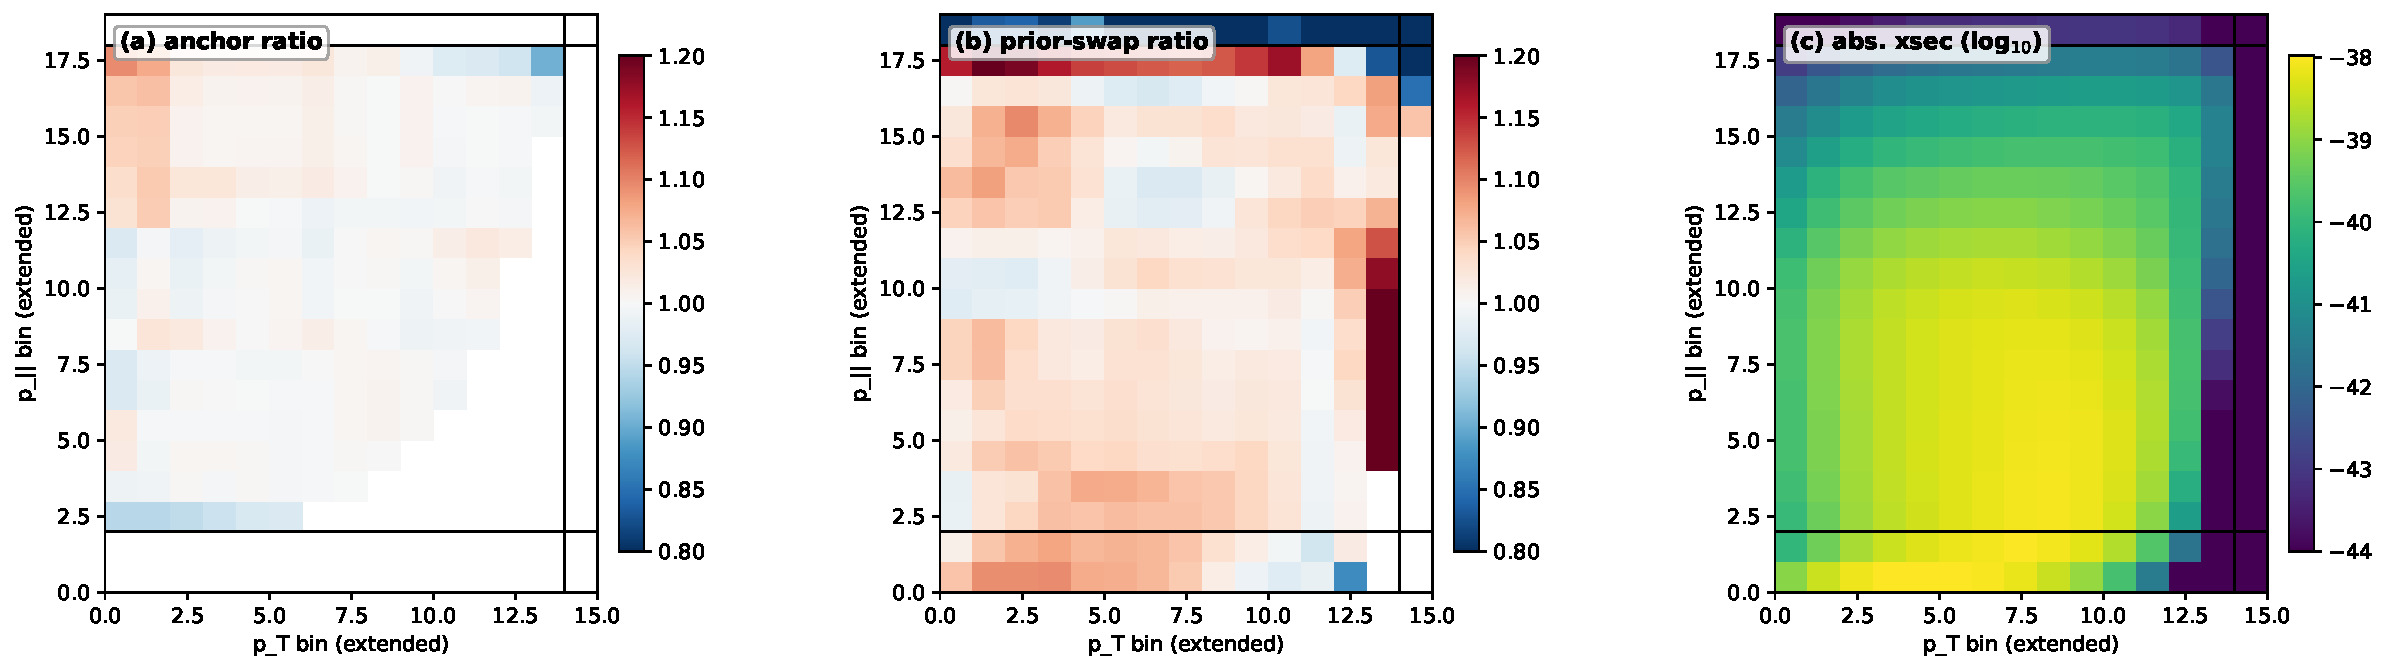
\includegraphics[width=0.99\textwidth]{fps_pilot_compare_MEFHC}
  \caption{The extended-fiducial scalar study, on the muon momentum grid
  ($p_T$ versus $p_\parallel$, in bin number). Left: inside the published region
  (between the black lines) the new result matches the original to better than
  one percent. Center: changing the starting simulation has a small effect in
  accepted cells but a much larger one in low-efficiency cells. Right: the
  preliminary central value over the enlarged truth domain (color = rate, on a
  logarithmic scale); detector-supported and prior-dominated regions must be
  interpreted separately.}
\end{figure}

\section{The takeaway}

% plain-language pass, director ruling on base defect F1 (DECISION-20261018-joseph-plain-language-pass; PLAIN-LANGUAGE.md C7)
Unbinned machine-learning unfolding reproduces a flagship MINERvA measurement
\emph{and} extends to many quantities at once without the larger response table
the binned method would need, although training, simulation and uncertainty
estimation still become more demanding. Using that, this analysis recovered a known low-recoil discrepancy with
a different unfolding method, exposed a localized central-value difference from the
MINERvA-tuned simulation, and
mapped a possible extension of the signal definition while exposing where the
detector provides too little information for a model-independent result.
% plain-language pass, review fix R9, RD13 (DECISION-20261018-joseph-plain-language-pass)
The multi-quantity measurements are shown as central values only: their error
bars have not been shown to be reliable, and end-to-end tests on simulation
show biases that are not included in their quoted uncertainty.
% plain-language pass 2 (DECISION-20261018-joseph-plain-language-pass2)
Separately, a joint test calibrated with simulated repeats of the whole analysis
rejects the hybrid hypotheses for all five tested simulations, overall and in
shape alone, at a combined five-percent error level. That holds only under
stated conditions: the test has no uncertainty for the calorimeter's response to
the hadronic recoil, convergence as its grid is refined has not been shown, and it does not
show that the five quantities together discriminate better than matched coarse
projections.
